% Compile-check for the generated tables at TMLR text width (6.5in). Used by reproduce_assets.sh.
\documentclass[10pt]{article}
\usepackage[letterpaper,textwidth=6.5in,textheight=9in]{geometry}
\usepackage{booktabs}
\usepackage{amsmath}
\usepackage{graphicx}
\begin{document}
% generated by scripts/build_paper_assets.py -- do not edit by hand
\begin{table*}[t]
\centering
\small
\setlength{\tabcolsep}{4pt}
\caption{LongMemEval-S held-out set (138 questions: 60 knowledge-update, 52 temporal, 26 abstention). Accuracy (\%) with 95\% bootstrap CIs over questions; stale-read = share of KU questions answered with the superseded value; tokens = mean reader prompt tokens. Async systems use the deterministic lag barrier with no reordering ($p_\text{ooo}=0$). Every cell is measured natively; the judge is qwen3.8-flash throughout.}
\label{tab:main138}
\begin{tabular}{lrcccccr}
\toprule
System & Lag & Overall & KU & Temporal & Abstention & Stale (\%) & Tokens \\
\midrule
\multicolumn{8}{l}{\textit{Reader: gemma4 (12B, local)}} \\
B1 sync (mutable) & 0 & 79.7\,{\scriptsize[72, 86]} & 83.3\,{\scriptsize[73, 92]} & 69.2\,{\scriptsize[56, 81]} & 92.3\,{\scriptsize[81, 100]} & 3.3 & 664 \\
B2 async & 1 & 23.2\,{\scriptsize[17, 30]} & 10.0\,{\scriptsize[3, 18]} & 3.8\,{\scriptsize[0, 10]} & 92.3\,{\scriptsize[81, 100]} & 68.3 & 656 \\
B3 recency (matched) & 1 & 58.0\,{\scriptsize[49, 66]} & 63.3\,{\scriptsize[52, 75]} & 32.7\,{\scriptsize[21, 46]} & 96.2\,{\scriptsize[88, 100]} & 30.0 & 1012 \\
Shadow v2 & 1 & 69.6\,{\scriptsize[62, 77]} & 80.0\,{\scriptsize[68, 90]} & 46.2\,{\scriptsize[33, 60]} & 92.3\,{\scriptsize[81, 100]} & 5.0 & 1204 \\
Lazy & 1 & 75.4\,{\scriptsize[68, 83]} & 76.7\,{\scriptsize[65, 87]} & 65.4\,{\scriptsize[52, 77]} & 92.3\,{\scriptsize[81, 100]} & 1.7 & 893 \\
DeltaWAL-Versioned & 0 & 83.3\,{\scriptsize[78, 89]} & 95.0\,{\scriptsize[88, 100]} & 65.4\,{\scriptsize[52, 77]} & 92.3\,{\scriptsize[81, 100]} & 1.7 & 791 \\
DeltaWAL-Versioned & 1 & 73.9\,{\scriptsize[67, 81]} & 88.3\,{\scriptsize[80, 95]} & 48.1\,{\scriptsize[35, 62]} & 92.3\,{\scriptsize[81, 100]} & 8.3 & 1255 \\
DeltaWAL-Versioned & 3 & 74.6\,{\scriptsize[67, 82]} & 88.3\,{\scriptsize[80, 95]} & 50.0\,{\scriptsize[37, 63]} & 92.3\,{\scriptsize[81, 100]} & 8.3 & 1266 \\
DeltaWAL-Versioned & 5 & 76.1\,{\scriptsize[69, 83]} & 91.7\,{\scriptsize[85, 98]} & 50.0\,{\scriptsize[37, 63]} & 92.3\,{\scriptsize[81, 100]} & 6.7 & 1288 \\
\midrule
\multicolumn{8}{l}{\textit{Reader: glm-5.3 (frontier, cloud)}} \\
B1 sync (mutable) & 0 & 81.9\,{\scriptsize[75, 88]} & 76.7\,{\scriptsize[65, 87]} & 82.7\,{\scriptsize[71, 92]} & 92.3\,{\scriptsize[81, 100]} & 0.0 & 664 \\
B2 async & 1 & 24.6\,{\scriptsize[17, 33]} & 11.7\,{\scriptsize[5, 20]} & 5.8\,{\scriptsize[0, 13]} & 92.3\,{\scriptsize[81, 100]} & 53.3 & 656 \\
B3 recency (matched) & 1 & 66.7\,{\scriptsize[59, 74]} & 80.0\,{\scriptsize[70, 90]} & 38.5\,{\scriptsize[25, 52]} & 92.3\,{\scriptsize[81, 100]} & 11.7 & 1012 \\
Shadow v2 & 1 & 84.8\,{\scriptsize[79, 91]} & 85.0\,{\scriptsize[75, 93]} & 80.8\,{\scriptsize[69, 90]} & 92.3\,{\scriptsize[81, 100]} & 0.0 & 1204 \\
Lazy & 1 & 82.6\,{\scriptsize[76, 88]} & 80.0\,{\scriptsize[68, 90]} & 80.8\,{\scriptsize[69, 92]} & 92.3\,{\scriptsize[81, 100]} & 0.0 & 893 \\
DeltaWAL-Versioned & 0 & 91.3\,{\scriptsize[86, 96]} & 96.7\,{\scriptsize[92, 100]} & 86.5\,{\scriptsize[77, 94]} & 88.5\,{\scriptsize[77, 100]} & 0.0 & 791 \\
DeltaWAL-Versioned & 1 & 91.3\,{\scriptsize[86, 96]} & 96.7\,{\scriptsize[92, 100]} & 86.5\,{\scriptsize[77, 94]} & 88.5\,{\scriptsize[77, 100]} & 0.0 & 1255 \\
DeltaWAL-Versioned & 3 & 91.3\,{\scriptsize[86, 96]} & 96.7\,{\scriptsize[92, 100]} & 86.5\,{\scriptsize[77, 94]} & 88.5\,{\scriptsize[77, 100]} & 0.0 & 1266 \\
\midrule
\multicolumn{8}{l}{\textit{Reader: gpt-6-luna (cloud)}} \\
B1 sync (mutable) & 0 & 81.2\,{\scriptsize[74, 88]} & 80.0\,{\scriptsize[70, 90]} & 78.8\,{\scriptsize[67, 88]} & 88.5\,{\scriptsize[77, 100]} & 3.3 & 664 \\
B2 async & 1 & 23.2\,{\scriptsize[16, 30]} & 11.7\,{\scriptsize[5, 20]} & 3.8\,{\scriptsize[0, 10]} & 88.5\,{\scriptsize[77, 100]} & 61.7 & 656 \\
B3 recency (matched) & 1 & 63.8\,{\scriptsize[56, 72]} & 71.7\,{\scriptsize[60, 82]} & 40.4\,{\scriptsize[27, 54]} & 92.3\,{\scriptsize[81, 100]} & 20.0 & 1012 \\
Shadow v2 & 1 & 81.9\,{\scriptsize[75, 88]} & 81.7\,{\scriptsize[72, 90]} & 76.9\,{\scriptsize[65, 88]} & 92.3\,{\scriptsize[81, 100]} & 1.7 & 1204 \\
Lazy & 1 & 79.0\,{\scriptsize[72, 86]} & 78.3\,{\scriptsize[67, 88]} & 73.1\,{\scriptsize[62, 85]} & 92.3\,{\scriptsize[81, 100]} & 0.0 & 893 \\
DeltaWAL-Versioned & 0 & 89.1\,{\scriptsize[84, 94]} & 93.3\,{\scriptsize[87, 98]} & 82.7\,{\scriptsize[73, 92]} & 92.3\,{\scriptsize[81, 100]} & 3.3 & 791 \\
DeltaWAL-Versioned & 1 & 88.4\,{\scriptsize[83, 93]} & 93.3\,{\scriptsize[87, 98]} & 80.8\,{\scriptsize[69, 90]} & 92.3\,{\scriptsize[81, 100]} & 3.3 & 1255 \\
DeltaWAL-Versioned & 3 & 88.4\,{\scriptsize[83, 93]} & 93.3\,{\scriptsize[87, 98]} & 80.8\,{\scriptsize[69, 90]} & 92.3\,{\scriptsize[81, 100]} & 3.3 & 1266 \\
\bottomrule
\end{tabular}
\end{table*}

\clearpage
% generated by scripts/build_paper_assets.py -- do not edit by hand
\begin{table*}[t]
\centering
\small
\setlength{\tabcolsep}{4pt}
\caption{History ablations on the 138 held-out questions. (a) Store policy and prompt format at lag 0: B1 sync (in-place, plain dated facts), the DeltaWAL prompt over its CAS store (in-place, epoch tags and precedence instruction), B1 sync over an append-only store with the same kind of epoch-tagged prompt, and DeltaWAL-Versioned (empty WAL); rows 2 and 3 differ only in the store, rows 1 and 2 only in the prompt. Pooled CIs resample questions. (b) Shadow v2 masking threshold, pooled over the five async cells (lag 1/3/5, $p_\text{ooo}\in\{0, 0.3\}$); re-run = question-cells whose set of masked facts differs from the frozen threshold's and therefore needed a new reader call (the others keep the frozen-threshold answer); `off' is the unmasked epoch-merge prompt on the same cells; CIs resample questions. (c) Out-of-order corruption (an updated key left at an older epoch) vs.\ missed merges, counted on the knowledge-update questions: the update's facts share no key with the earlier evidence, so no keyed policy can supersede the old value.}
\label{tab:history}
\begin{tabular}{llccc}
\toprule
\multicolumn{5}{l}{\textbf{(a) Write side at lag 0: store policy and prompt format}} \\
\midrule
Store & Prompt & \begin{tabular}[b]{@{}c@{}}KU-past, pooled\\($n$=13 per reader)\end{tabular} & \begin{tabular}[b]{@{}c@{}}KU-past per reader\\(gemma4 / glm / gpt)\end{tabular} & \begin{tabular}[b]{@{}c@{}}KU-current, pooled\\($n$=47 per reader)\end{tabular} \\
\midrule
in-place & plain (B1) & 43.6\,{\scriptsize[21, 69]} & 46.2 / 38.5 / 46.2 & 90.1\,{\scriptsize[83, 96]} \\
in-place & epoch tags (DeltaWAL prompt) & 46.2\,{\scriptsize[23, 69]} & 46.2 / 46.2 / 46.2 & 92.9\,{\scriptsize[87, 99]} \\
append-only & epoch tags (B1 versioned) & 97.4\,{\scriptsize[92, 100]} & 92.3 / 100.0 / 100.0 & 94.3\,{\scriptsize[88, 99]} \\
append-only & epoch tags (DeltaWAL-V.) & 97.4\,{\scriptsize[92, 100]} & 92.3 / 100.0 / 100.0 & 94.3\,{\scriptsize[89, 99]} \\
\bottomrule
\end{tabular}
\par\medskip
\begin{tabular}{lrcccc}
\toprule
\multicolumn{6}{l}{\textbf{(b) Read side: Shadow v2 masking threshold (gemma4; frozen 0.72)}} \\
\midrule
Threshold & Re-run & Overall & KU & KU-past & KU-current \\
\midrule
0.60 & 521 & 65.5\,{\scriptsize[58, 73]} & 75.0\,{\scriptsize[63, 85]} & 15.4\,{\scriptsize[0, 38]} & 91.5\,{\scriptsize[83, 98]} \\
0.65 & 406 & 68.1\,{\scriptsize[61, 76]} & 77.7\,{\scriptsize[67, 88]} & 27.7\,{\scriptsize[8, 51]} & 91.5\,{\scriptsize[83, 98]} \\
0.70 & 170 & 70.3\,{\scriptsize[63, 78]} & 80.0\,{\scriptsize[70, 90]} & 30.8\,{\scriptsize[8, 54]} & 93.6\,{\scriptsize[87, 100]} \\
0.72 & 0 & 70.4\,{\scriptsize[63, 78]} & 79.3\,{\scriptsize[69, 88]} & 41.5\,{\scriptsize[15, 68]} & 89.8\,{\scriptsize[81, 97]} \\
0.75 & 183 & 71.7\,{\scriptsize[64, 79]} & 83.0\,{\scriptsize[73, 91]} & 58.5\,{\scriptsize[31, 85]} & 89.8\,{\scriptsize[81, 97]} \\
off (unmasked) & -- & 74.5\,{\scriptsize[68, 81]} & 87.3\,{\scriptsize[79, 95]} & 84.6\,{\scriptsize[62, 100]} & 88.1\,{\scriptsize[79, 96]} \\
\bottomrule
\end{tabular}
\par\medskip
\begin{tabular}{rlrrrr}
\toprule
\multicolumn{6}{l}{\textbf{(c) Store integrity under reordering ($p_\text{ooo}=0.3$, store-level)}} \\
\midrule
Lag & Store policy & \begin{tabular}[b]{@{}c@{}}Updated\\keys\end{tabular} & \begin{tabular}[b]{@{}c@{}}Corrupted\\keys (OOCR)\end{tabular} & \begin{tabular}[b]{@{}c@{}}CAS\\rejections\end{tabular} & \begin{tabular}[b]{@{}c@{}}KU questions with\\missed merge\end{tabular} \\
\midrule
1 & LWW (B2, B3) & 294 & 23 (7.8\%) & 0 & 9/60 (15.0\%) \\
1 & CAS-fenced (DeltaWAL) & 294 & 0 (0.0\%) & 25 & 9/60 (15.0\%) \\
3 & LWW (B2, B3) & 267 & 24 (9.0\%) & 0 & 11/60 (18.3\%) \\
3 & CAS-fenced (DeltaWAL) & 267 & 0 (0.0\%) & 26 & 11/60 (18.3\%) \\
\bottomrule
\end{tabular}
\end{table*}

\clearpage
% generated by scripts/build_paper_assets.py -- do not edit by hand
\begin{table*}[t]
\centering
\small
\setlength{\tabcolsep}{4pt}
\caption{Non-update regression: 60 LongMemEval-S questions disjoint from the held-out set. The extractor sees assistant turns truncated to 300 characters, so fact-only memories rarely contain assistant-provided details (SS-assistant); DeltaWAL recovers them from the raw WAL turn when the session is in flight. SS-preference uses LongMemEval's rubric grading. glm-5.3 was run only on the B1 and DeltaWAL-Versioned cells.}
\label{tab:regression60}
\begin{tabular}{lrcccccr}
\toprule
System & Lag & \begin{tabular}[b]{@{}c@{}}All\\($n$=60)\end{tabular} & \begin{tabular}[b]{@{}c@{}}Multi-session\\($n$=30)\end{tabular} & \begin{tabular}[b]{@{}c@{}}SS-user\\($n$=10)\end{tabular} & \begin{tabular}[b]{@{}c@{}}SS-assistant\\($n$=10)\end{tabular} & \begin{tabular}[b]{@{}c@{}}SS-preference\\($n$=10)\end{tabular} & Tokens \\
\midrule
\multicolumn{8}{l}{\textit{Reader: gemma4 (12B, local)}} \\
B1 sync (mutable) & 0 & 40.0\,{\scriptsize[28, 53]} & 36.7\,{\scriptsize[20, 53]} & 90.0\,{\scriptsize[70, 100]} & 10.0\,{\scriptsize[0, 30]} & 30.0\,{\scriptsize[0, 60]} & 653 \\
DeltaWAL-Versioned & 0 & 46.7\,{\scriptsize[35, 60]} & 53.3\,{\scriptsize[37, 73]} & 90.0\,{\scriptsize[70, 100]} & 10.0\,{\scriptsize[0, 30]} & 20.0\,{\scriptsize[0, 50]} & 778 \\
B2 async & 1 & 10.0\,{\scriptsize[3, 18]} & 16.7\,{\scriptsize[7, 30]} & 0.0\,{\scriptsize[0, 0]} & 0.0\,{\scriptsize[0, 0]} & 10.0\,{\scriptsize[0, 30]} & 654 \\
B3 recency (matched) & 1 & 46.7\,{\scriptsize[33, 60]} & 46.7\,{\scriptsize[30, 67]} & 70.0\,{\scriptsize[40, 100]} & 20.0\,{\scriptsize[0, 50]} & 50.0\,{\scriptsize[20, 80]} & 1003 \\
DeltaWAL-Versioned & 1 & 65.0\,{\scriptsize[53, 77]} & 53.3\,{\scriptsize[37, 73]} & 90.0\,{\scriptsize[70, 100]} & 80.0\,{\scriptsize[50, 100]} & 60.0\,{\scriptsize[30, 90]} & 1375 \\
\midrule
\multicolumn{8}{l}{\textit{Reader: gpt-6-luna (cloud)}} \\
B1 sync (mutable) & 0 & 55.0\,{\scriptsize[42, 68]} & 50.0\,{\scriptsize[33, 67]} & 90.0\,{\scriptsize[70, 100]} & 10.0\,{\scriptsize[0, 30]} & 80.0\,{\scriptsize[50, 100]} & 653 \\
DeltaWAL-Versioned & 0 & 66.7\,{\scriptsize[55, 78]} & 73.3\,{\scriptsize[57, 87]} & 90.0\,{\scriptsize[70, 100]} & 0.0\,{\scriptsize[0, 0]} & 90.0\,{\scriptsize[70, 100]} & 778 \\
B2 async & 1 & 8.3\,{\scriptsize[2, 15]} & 16.7\,{\scriptsize[3, 30]} & 0.0\,{\scriptsize[0, 0]} & 0.0\,{\scriptsize[0, 0]} & 0.0\,{\scriptsize[0, 0]} & 654 \\
B3 recency (matched) & 1 & 60.0\,{\scriptsize[48, 72]} & 63.3\,{\scriptsize[47, 80]} & 70.0\,{\scriptsize[40, 100]} & 20.0\,{\scriptsize[0, 50]} & 80.0\,{\scriptsize[50, 100]} & 1003 \\
DeltaWAL-Versioned & 1 & 71.7\,{\scriptsize[60, 83]} & 70.0\,{\scriptsize[53, 87]} & 90.0\,{\scriptsize[70, 100]} & 70.0\,{\scriptsize[40, 100]} & 60.0\,{\scriptsize[30, 90]} & 1375 \\
\midrule
\multicolumn{8}{l}{\textit{Reader: glm-5.3 (frontier, cloud)}} \\
B1 sync (mutable) & 0 & 58.3\,{\scriptsize[45, 70]} & 60.0\,{\scriptsize[43, 77]} & 80.0\,{\scriptsize[50, 100]} & 10.0\,{\scriptsize[0, 30]} & 80.0\,{\scriptsize[50, 100]} & 653 \\
DeltaWAL-Versioned & 0 & 68.3\,{\scriptsize[57, 80]} & 73.3\,{\scriptsize[57, 90]} & 90.0\,{\scriptsize[70, 100]} & 10.0\,{\scriptsize[0, 30]} & 90.0\,{\scriptsize[70, 100]} & 778 \\
DeltaWAL-Versioned & 1 & 80.0\,{\scriptsize[70, 90]} & 73.3\,{\scriptsize[57, 90]} & 90.0\,{\scriptsize[70, 100]} & 80.0\,{\scriptsize[50, 100]} & 90.0\,{\scriptsize[70, 100]} & 1375 \\
\bottomrule
\end{tabular}
\end{table*}

\clearpage
% generated by scripts/build_paper_assets.py -- do not edit by hand
\begin{table*}[t]
\centering
\small
\setlength{\tabcolsep}{4pt}
\caption{Mem0 OSS 1.0.11 (classic ADD/UPDATE/DELETE write path) on the 60 held-out knowledge-update questions. Mem0 sync ingests every session; Mem0 async leaves the final (update) session in flight; Mem0 + DeltaWAL adds the epoch-tagged WAL and relevance gate ($\tau=0.35$) on top of the async store. The history hook renders, for every retrieved memory, its earlier versions from \texttt{Memory.history()} in epoch order (run on the KU-past questions only; $^\ast$stale rate over those questions). On the 13 KU-past questions Mem0 updated the older evidence memory in place in 11 and deleted it in 0.}
\label{tab:mem0}
\begin{tabular}{lrcccc}
\toprule
System & Lag & \begin{tabular}[b]{@{}c@{}}KU\\($n$=60)\end{tabular} & \begin{tabular}[b]{@{}c@{}}KU-past\\($n$=13)\end{tabular} & \begin{tabular}[b]{@{}c@{}}KU-current\\($n$=47)\end{tabular} & \begin{tabular}[b]{@{}c@{}}Stale\\(\%)\end{tabular} \\
\midrule
\multicolumn{6}{l}{\textit{Reader: gemma4 (12B, local)}} \\
Mem0 sync & 0 & 76.7\,{\scriptsize[65, 87]} & 46.1\,{\scriptsize[23, 69]} & 85.1\,{\scriptsize[74, 94]} & 6.7 \\
Mem0 async & 1 & 10.0\,{\scriptsize[3, 18]} & 46.1\,{\scriptsize[23, 77]} & 0.0\,{\scriptsize[0, 0]} & 66.7 \\
Mem0 + DeltaWAL & 1 & 91.7\,{\scriptsize[83, 98]} & 92.3\,{\scriptsize[77, 100]} & 91.5\,{\scriptsize[83, 98]} & 6.7 \\
Mem0 sync + history hook & 0 & -- & 100.0\,{\scriptsize[100, 100]} & -- & 0.0$^\ast$ \\
\midrule
\multicolumn{6}{l}{\textit{Reader: gpt-6-luna (cloud)}} \\
Mem0 sync & 0 & 76.7\,{\scriptsize[65, 87]} & 53.9\,{\scriptsize[31, 77]} & 83.0\,{\scriptsize[72, 94]} & 6.7 \\
Mem0 async & 1 & 11.7\,{\scriptsize[5, 20]} & 53.9\,{\scriptsize[31, 85]} & 0.0\,{\scriptsize[0, 0]} & 63.3 \\
Mem0 + DeltaWAL & 1 & 96.7\,{\scriptsize[92, 100]} & 100.0\,{\scriptsize[100, 100]} & 95.7\,{\scriptsize[89, 100]} & 1.7 \\
Mem0 sync + history hook & 0 & -- & 100.0\,{\scriptsize[100, 100]} & -- & 0.0$^\ast$ \\
\midrule
\multicolumn{6}{l}{\textit{Reader: glm-5.3 (frontier, cloud)}} \\
Mem0 sync & 0 & 76.7\,{\scriptsize[65, 87]} & 46.1\,{\scriptsize[23, 69]} & 85.1\,{\scriptsize[74, 94]} & 5.0 \\
Mem0 + DeltaWAL & 1 & 96.7\,{\scriptsize[92, 100]} & 100.0\,{\scriptsize[100, 100]} & 95.7\,{\scriptsize[89, 100]} & 0.0 \\
Mem0 sync + history hook & 0 & -- & 100.0\,{\scriptsize[100, 100]} & -- & 0.0$^\ast$ \\
\bottomrule
\end{tabular}
\par\medskip
\begin{tabular}{lrrr}
\toprule
Mem0 history events (60 questions) & ADD & UPDATE & DELETE \\
\midrule
sessions $1..T{-}1$ (async view) & 6913 & 152 & 3 \\
sessions $1..T$ (sync view) & 7125 & 265 & 5 \\
KU-past subset, sessions $1..T$ ($n$=13) & 1539 & 52 & 0 \\
\bottomrule
\end{tabular}
\end{table*}

\clearpage
% generated by scripts/build_paper_assets.py -- do not edit by hand
\begin{table*}[t]
\centering
\small
\setlength{\tabcolsep}{4pt}
\caption{MemConflict (90 questions, 30/30/30 dynamic/static/conditional). A pre-evaluation audit of 30 questions sampled from the whole pool (LLM reading agent) found 29/30 clean; the later full audit of these evaluated questions found fewer and misses the $\geq$85\% gate (Section~\ref{sec:memconflict}, Table~\ref{tab:memconflict_clean}). `Static: believed false' = static questions answered with the later, false statement. In the async cells the false statement sits in the in-flight session, which B2/B3 never see.}
\label{tab:memconflict}
\begin{tabular}{lrccccc}
\toprule
System & Lag & \begin{tabular}[b]{@{}c@{}}All\\($n$=90)\end{tabular} & \begin{tabular}[b]{@{}c@{}}Dynamic\\($n$=30)\end{tabular} & \begin{tabular}[b]{@{}c@{}}Static\\($n$=30)\end{tabular} & \begin{tabular}[b]{@{}c@{}}Conditional\\($n$=30)\end{tabular} & \begin{tabular}[b]{@{}c@{}}Static: believed\\false statement\end{tabular} \\
\midrule
\multicolumn{7}{l}{\textit{Reader: gemma4 (12B, local)}} \\
B1 sync (mutable) & 0 & 36.7\,{\scriptsize[27, 47]} & 40.0\,{\scriptsize[23, 57]} & 30.0\,{\scriptsize[13, 47]} & 40.0\,{\scriptsize[23, 60]} & 50.0\,{\scriptsize[33, 67]} \\
DeltaWAL-Versioned & 0 & 40.0\,{\scriptsize[30, 50]} & 50.0\,{\scriptsize[33, 67]} & 20.0\,{\scriptsize[7, 33]} & 50.0\,{\scriptsize[33, 70]} & 80.0\,{\scriptsize[67, 93]} \\
B2 async & 1 & 46.7\,{\scriptsize[36, 58]} & 16.7\,{\scriptsize[3, 30]} & 76.7\,{\scriptsize[60, 90]} & 46.7\,{\scriptsize[30, 63]} & 3.3\,{\scriptsize[0, 10]} \\
B3 recency (matched) & 1 & 50.0\,{\scriptsize[40, 61]} & 13.3\,{\scriptsize[3, 27]} & 76.7\,{\scriptsize[60, 90]} & 60.0\,{\scriptsize[43, 77]} & 6.7\,{\scriptsize[0, 17]} \\
DeltaWAL-Versioned & 1 & 47.8\,{\scriptsize[38, 59]} & 46.7\,{\scriptsize[30, 63]} & 40.0\,{\scriptsize[23, 57]} & 56.7\,{\scriptsize[40, 77]} & 50.0\,{\scriptsize[33, 67]} \\
\midrule
\multicolumn{7}{l}{\textit{Reader: gpt-6-luna (cloud)}} \\
B1 sync (mutable) & 0 & 36.7\,{\scriptsize[27, 47]} & 36.7\,{\scriptsize[20, 53]} & 33.3\,{\scriptsize[17, 50]} & 40.0\,{\scriptsize[23, 57]} & 53.3\,{\scriptsize[37, 70]} \\
DeltaWAL-Versioned & 0 & 45.6\,{\scriptsize[36, 57]} & 56.7\,{\scriptsize[40, 73]} & 23.3\,{\scriptsize[10, 40]} & 56.7\,{\scriptsize[40, 73]} & 66.7\,{\scriptsize[50, 83]} \\
B2 async & 1 & 47.8\,{\scriptsize[38, 58]} & 13.3\,{\scriptsize[3, 27]} & 76.7\,{\scriptsize[60, 90]} & 53.3\,{\scriptsize[37, 70]} & 6.7\,{\scriptsize[0, 17]} \\
B3 recency (matched) & 1 & 45.6\,{\scriptsize[34, 56]} & 20.0\,{\scriptsize[7, 33]} & 70.0\,{\scriptsize[53, 87]} & 46.7\,{\scriptsize[30, 63]} & 20.0\,{\scriptsize[7, 37]} \\
DeltaWAL-Versioned & 1 & 47.8\,{\scriptsize[38, 58]} & 60.0\,{\scriptsize[43, 77]} & 40.0\,{\scriptsize[23, 57]} & 43.3\,{\scriptsize[27, 63]} & 56.7\,{\scriptsize[40, 73]} \\
\midrule
\multicolumn{7}{l}{\textit{Reader: glm-5.3-flash (cloud)}} \\
B1 sync (mutable) & 0 & 40.0\,{\scriptsize[30, 50]} & 50.0\,{\scriptsize[33, 67]} & 30.0\,{\scriptsize[13, 47]} & 40.0\,{\scriptsize[23, 57]} & 53.3\,{\scriptsize[37, 70]} \\
DeltaWAL-Versioned & 0 & 47.8\,{\scriptsize[38, 58]} & 53.3\,{\scriptsize[37, 70]} & 30.0\,{\scriptsize[13, 47]} & 60.0\,{\scriptsize[43, 77]} & 63.3\,{\scriptsize[47, 80]} \\
B2 async & 1 & 44.4\,{\scriptsize[34, 56]} & 16.7\,{\scriptsize[7, 30]} & 70.0\,{\scriptsize[53, 87]} & 46.7\,{\scriptsize[30, 63]} & 10.0\,{\scriptsize[0, 23]} \\
B3 recency (matched) & 1 & 46.7\,{\scriptsize[37, 57]} & 20.0\,{\scriptsize[7, 33]} & 70.0\,{\scriptsize[53, 87]} & 50.0\,{\scriptsize[33, 67]} & 13.3\,{\scriptsize[3, 27]} \\
DeltaWAL-Versioned & 1 & 45.6\,{\scriptsize[34, 56]} & 56.7\,{\scriptsize[40, 73]} & 26.7\,{\scriptsize[10, 43]} & 53.3\,{\scriptsize[33, 73]} & 63.3\,{\scriptsize[43, 80]} \\
\bottomrule
\end{tabular}
\end{table*}

\clearpage
% generated by scripts/build_paper_assets.py -- do not edit by hand
\begin{table*}[t]
\centering
\small
\setlength{\tabcolsep}{4pt}
\caption{Wall-clock latency (ms) on the real stack (Redpanda, Redis, PostgreSQL/pgvector, local qwen3-embedding:0.6b embeddings), 10 dev questions at lag 3; write ack over 416 sessions, read paths exclude the reader decode. B1 acknowledges only after synchronous extraction (recorded live extractor time), embedding and upsert; B2 after the broker ack; DeltaWAL after the Redis WAL write-through and broker ack. Cold = the WAL tail is embedded at read time; Lazy runs a live extraction call per query. DeltaWAL-Versioned uses the DeltaWAL read path.}
\label{tab:latency}
\begin{tabular}{lrrrrrr}
\toprule
System & \multicolumn{2}{c}{Write ack} & \multicolumn{2}{c}{Read (incl.\ query emb.)} & \multicolumn{2}{c}{Read (excl.\ query emb.)} \\
\cmidrule(lr){2-3}\cmidrule(lr){4-5}\cmidrule(lr){6-7}
 & p50 & p95 & p50 & p95 & p50 & p95 \\
\midrule
B1 sync & 10,168 & 23,810 & 18.6 & 20.7 & 4.21 & 5.26 \\
B2 async & 0.98 & 4.60 & 16.1 & 17.4 & 4.09 & 4.74 \\
DeltaWAL (warm) & 2.67 & 7.34 & 21.3 & 26.7 & 10.6 & 14.6 \\
DeltaWAL (cold) & 2.67 & 7.34 & -- & -- & 429.6 & 495.0 \\
Shadow v2 (warm) & 2.67 & 7.34 & 21.7 & 23.3 & 10.8 & 12.4 \\
Shadow v2 (cold) & 2.67 & 7.34 & -- & -- & 492.4 & 681.3 \\
Lazy & 2.67 & 7.34 & 3,711 & 9,441 & 3,699 & 9,430 \\
\bottomrule
\end{tabular}
\end{table*}

\clearpage
\begin{figure*}[t]\centering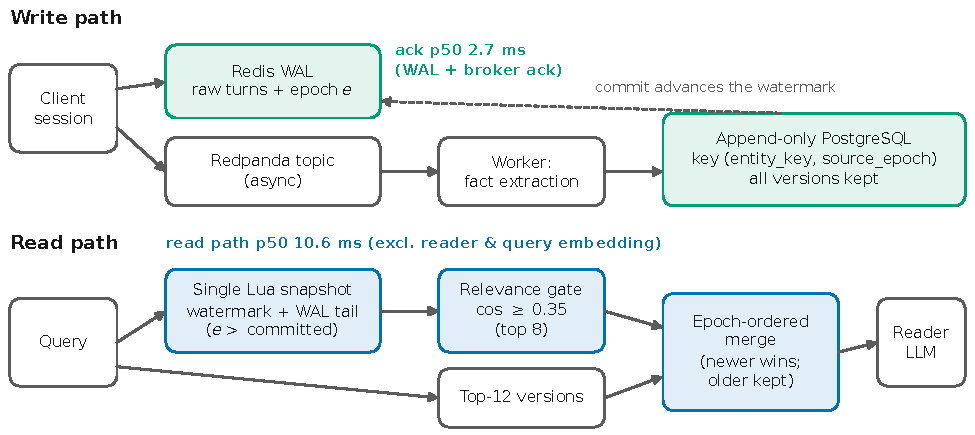
\includegraphics[width=\textwidth]{figures/fig1_architecture.pdf}\caption{fig1}\end{figure*}
\begin{figure*}[t]\centering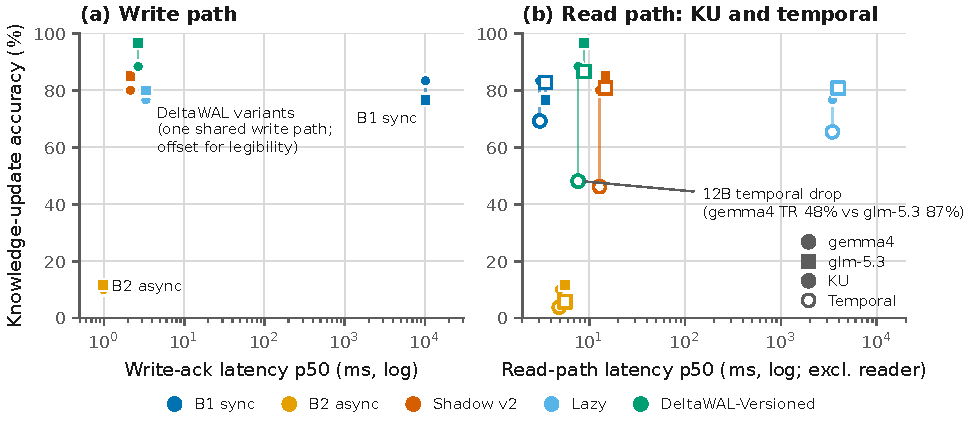
\includegraphics[width=\textwidth]{figures/fig2_pareto.pdf}\caption{fig2}\end{figure*}
\clearpage
\begin{figure*}[t]\centering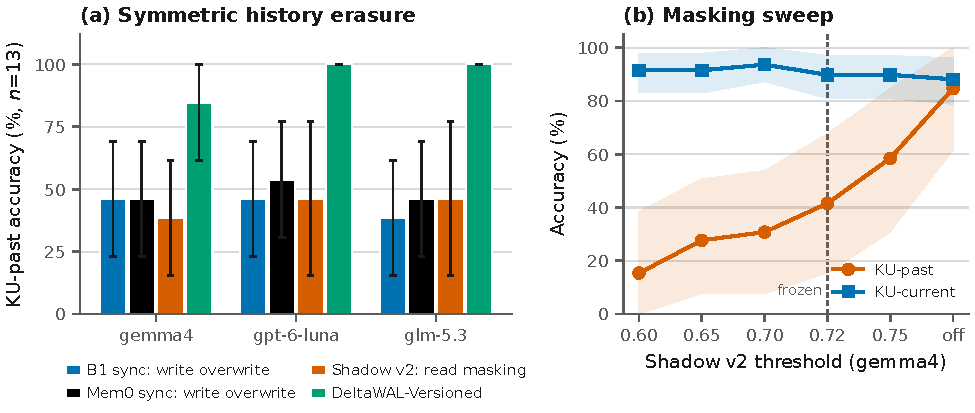
\includegraphics[width=\textwidth]{figures/fig3_destructive_symmetry.pdf}\caption{fig3}\end{figure*}
\begin{figure*}[t]\centering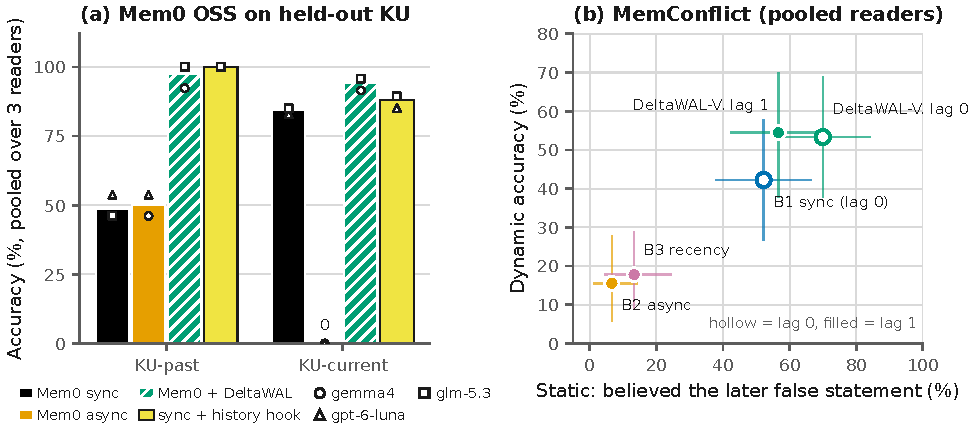
\includegraphics[width=\textwidth]{figures/fig4_external.pdf}\caption{fig4}\end{figure*}
\end{document}
